%%
% Figure of the three fits for each of the two years.
%


\begin{figure}
  \centering
  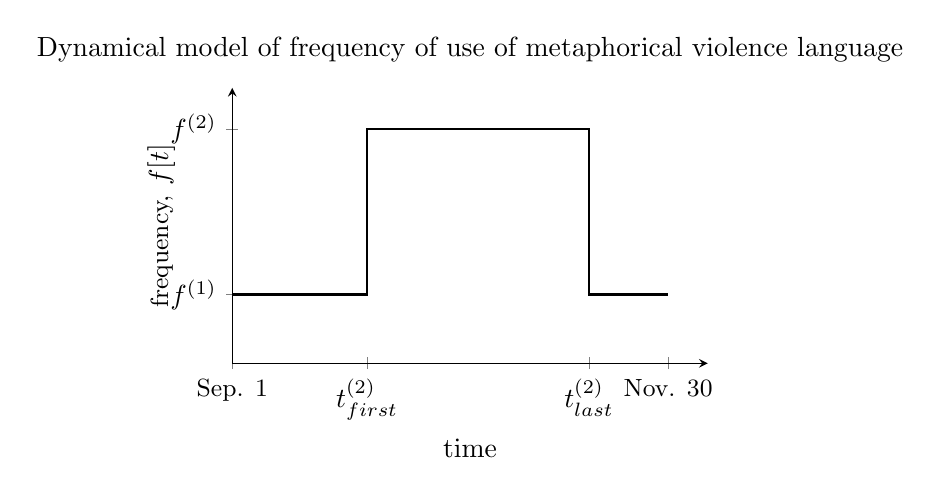
\begin{tikzpicture}
    \begin{axis}[%
      ,xlabel=time
      ,ylabel={{\small frequency,} $f[t]$}
      ,axis x line = bottom,axis y line = left
      ,xmax=3.25
      ,xtick={0.25, 1.1, 2.5, 3}
      ,xticklabels={{\small Sep. 1}, $t_{first}^{(2)}$, $t_{last}^{(2)}$, {\small Nov. 30}}
      ,ytick={.5, 1.7}
      ,y label style={at={(axis description cs:-0.10,.5)}}
      ,yticklabels={$f^{(1)}$, $f^{(2)}$}
      ,ymax=2.0 % or enlarge y limits=upper
      ,ymin=0.0
      ,title={Dynamical model of frequency of use of metaphorical violence language}
      ,width=3.0in
      ,height=2.0in
      ]
      \addplot+[const plot, no marks, thick, black] coordinates {(0.25,.5) (1.1,1.7) (2.5,.5) (3, .5)};
    \end{axis}
  \end{tikzpicture}
  \caption{Illustration of the dynamical model of Equation 1. 
    We determine $t^{(2)}_{first}$, $t^{(2)}_{last}$, $f^{(1)}$, and $f^{(2)}$
    for six time series (two shows on three networks in 2012 and 2016) 
    through Bayesian inference. 
    }
  \label{fig:model-illustration}
\end{figure}


% \begin{figure}
  \centering
  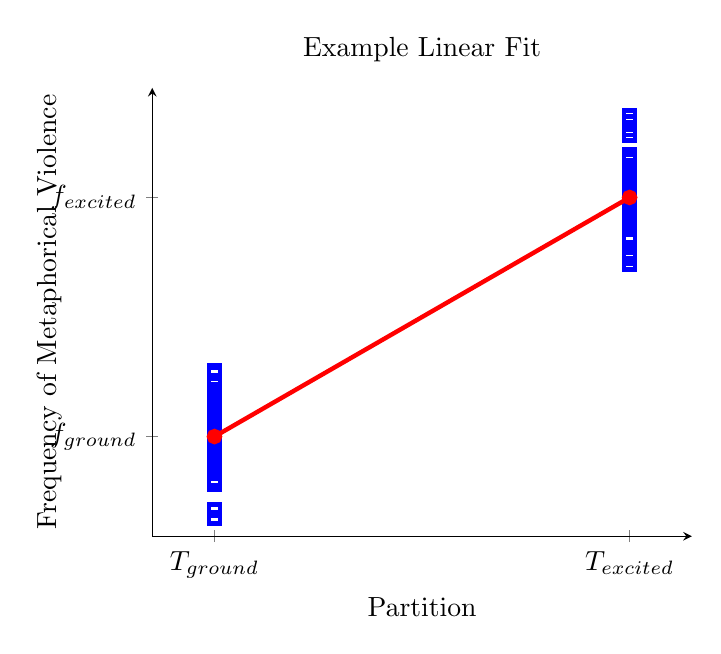
\begin{tikzpicture}
    \begin{axis}[
      ,title=Example Linear Fit
      ,axis x line = bottom, axis y line = left
      ,xlabel=Partition
      ,y label style={at={(axis description cs:-0.15,.5)}}
      ,ylabel=Frequency of Metaphorical Violence
      ,xmin=-.15, xmax=1.15
      ,ymin=0, ymax=2.25
      ,xtick={0, 1}
      ,xticklabels={$T_{ground}$, $T_{excited}$}
      ,ytick={0.5, 1.7} 
      ,yticklabels={$f_{ground}$, $f_{excited}$}
      ,every axis plot/.append style={ultra thick}
      ,clip marker paths=true
      ,anchor=origin
      ]
      \addplot+[only marks, mark=square, blue] coordinates {
        (0, 0.28176763326) (0, 0.350579774235) (0, 0.494762486627) (0, 0.698017229947) (0, 0.0914119670018) (0, 0.562791554989) (0, 0.414408243237) (0, 0.448752389982) (0, 0.534869456009) (0, 0.565298122439) (0, 0.713342069417) (0, 0.570802600869) (0, 0.600080420076) (0, 0.339212985545) (0, 0.536222381064) (0, 0.325157942968) (0, 0.482143784654) (0, 0.651252469343) (0, 0.262656739438) (0, 0.734264833239) (0, 0.527160094444) (0, 0.670540313522) (0, 0.782590258513) (0, 0.544998389383) (0, 0.406587061347) (0, 0.13090649078) (0, 0.325595587657) (0, 0.467227203324) (0, 0.26067945992) (0, 0.42655727858) (0, 0.280874951953) (0, 0.627523159582) (0, 0.52163666621) (0, 0.689592043265) (0, 0.582769397727) (0, 0.707024689504) (0, 0.598615409781) (0, 0.347973302243) (0, 0.360956698235) (0, 0.699323678165) (0, 0.819275219019) (0, 0.832535941995) (0, 0.572485985687) (0, 0.727924580262) (0, 0.41724329832) };
      \addplot+[only marks, mark=square, blue] coordinates {
        (1.0, 1.91247092918) (1.0, 1.5394596921) (1.0, 2.10773281394) (1.0, 1.89887130293) (1.0, 1.61425294087) (1.0, 1.71383269787) (1.0, 1.8310274463) (1.0, 1.73530670109) (1.0, 1.40727197112) (1.0, 1.82023604091) (1.0, 1.63965557868) (1.0, 1.73899638436) (1.0, 1.36919392698) (1.0, 1.58641297881) (1.0, 1.83803888564) (1.0, 1.71802566345) (1.0, 1.68759269019) (1.0, 2.01343061625) (1.0, 1.60507200871) (1.0, 1.79480251021) (1.0, 1.36483678083) (1.0, 1.85793134182) (1.0, 1.56941110605) (1.0, 1.4855004683) (1.0, 1.76177910132) (1.0, 1.58485972151) (1.0, 1.5846086847) (1.0, 1.48354037111) (1.0, 2.04198439011) (1.0, 1.6987951821) (1.0, 1.44801569567) (1.0, 2.07846405613) (1.0, 1.80107745091) (1.0, 1.3956308386) (1.0, 1.62193882796) (1.0, 1.55818973594) (1.0, 1.8896926668) (1.0, 1.71657899717) (1.0, 1.58108619149) (1.0, 1.59786892921) (1.0, 1.66832037628) (1.0, 1.83181642753) (1.0, 1.79348201084) (1.0, 1.88734472296) (1.0, 1.62566264372)
      };
      \addplot+[red] coordinates { (0, .5) (1.0, 1.7) };
    \end{axis}
  \end{tikzpicture}
  \caption{Each model corresponding to a pair of partition times, $(\tau_1^*, \tau_2^*)$,
  is a linear fit. The linear model that minimizes the AIC is considered the
  most likely to minimize information loss. We fit about 1,000 linear models
  to the coded data just like this one. Once the optimal pair $(\tau_1^*, \tau_2^*)$
  has been identified, we obtain $f_{ground}$ and $f_{excited}$ as identified in the linear fit.
  }
\label{fig:linear-model-illustration}
\end{figure}


\begin{figure}[!htb]
  \centering
  \begin{subfigure}{0.8\linewidth}
    \centering
    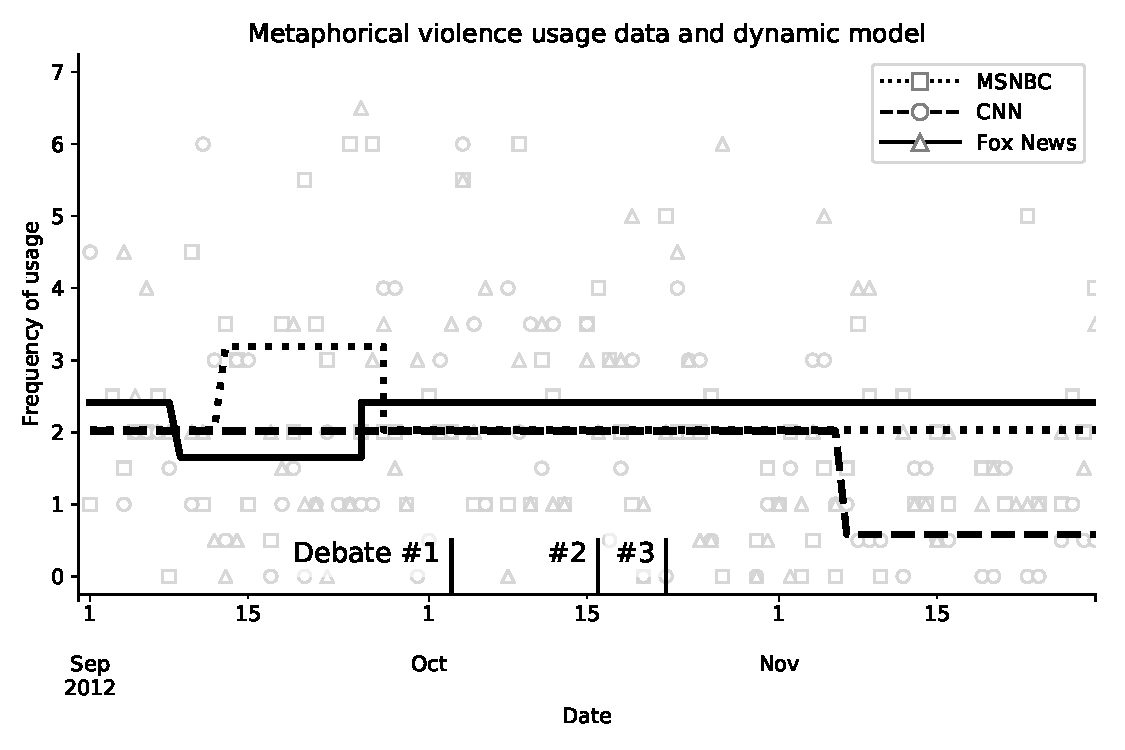
\includegraphics[width=\textwidth]{Figures/ModelFits-2012.pdf}
   \caption{\quad2012}
    \label{fig:ModelFits-2012}
  \end{subfigure}
  \begin{subfigure}{0.8\linewidth}
    \centering
    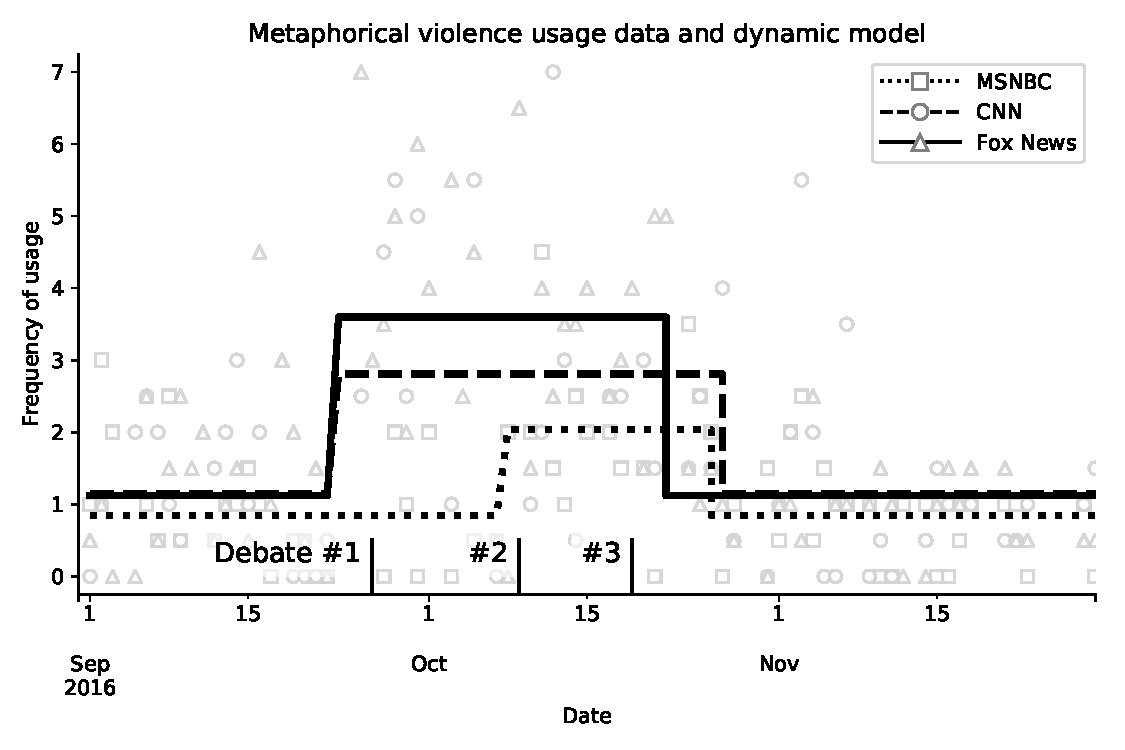
\includegraphics[width=\textwidth]{Figures/ModelFits-2016.pdf}
   \caption{\quad2016}
    \label{fig:ModelFits-2016}
  \end{subfigure}

  \caption{Observed daily frequencies (markers) and best-fit models (lines).
    The dynamical impulse model is given in 
    Equation 1. In four of the six network-year pairs, 
    there is an increase in the frequency of metaphorical violence language in the
    three-month study period: MSNBC in 2012 and all three networks in 2016. 
    However, two of the six network-year pairs showed decreases in frequency
    of metaphorical violence language use in one three-month period: CNN and Fox News
    in 2012. 
  } 
  \label{fig:ModelFits}
\end{figure}


\begin{table}
  \centering
  \bgroup
    \begin{subtable}{\textwidth}
      \centering
      \begin{tabular}{lr}
        \toprule
        Show (Network) & Total Uses \\
        \midrule
        The Rachel Maddow Show (MSNBC) & 93 \\
        Hardball With Chris Matthews (MSNBC) & 208 \\
        Anderson Cooper 360 (CNN) & 99 \\
        Piers Morgan Tonight (CNN) & 118 \\
        The O'Reilly Factor (Fox News) & 141 \\
        Hannity (Fox News) & 133 \\
        \bottomrule
      \end{tabular}
      \caption{Total number of uses metaphorical violence language by news show in 2012}
      \label{tab:by-show-2012}
    \end{subtable} \\  \vspace{1.5em}
    \begin{subtable}{\textwidth}
      \centering
      \begin{tabular}{lr}
        \toprule
        Show (Network) & Total Uses \\
        \midrule
        The Rachel Maddow Show (MSNBC) & 66 \\
        The Last Word with Lawrence O'Donnel (MSNBC) & 80 \\
        Anderson Cooper 360 (CNN) & 100 \\
        Erin Burnett OutFront (CNN) & 118 \\
        The O'Reilly Factor (Fox News) & 146 \\
        The Kelly File (Fox News) & 148 \\
        \bottomrule
      \end{tabular} \quad
      \caption{Total number of uses metaphorical violence language by news show in 2016}
      \label{tab:by-show-2016}
    \end{subtable}
  \egroup
  \caption{Total uses by show in each of the two study years}
  \label{tab:by-show}
\end{table}


%%
% Table with network and violent words
%
\begin{table}[h]
  \centering

  \begin{subtable}{\linewidth}
    \centering
    \begin{tabular}{llrrrr}
\toprule
       &     & $f^{(1)}$ & $f^{(2)}$ & \emph{delta} & total uses \\
Violent Word & Network &           &           &            &            \\
\midrule
hit & MSNBC &      0.86 &      0.86 &      -0.00 &         67 \\
       & CNN &      0.54 &      0.11 &      -0.81 &         34 \\
       & Fox News &      0.57 &      0.33 &      -0.42 &         41 \\
\hline
beat & MSNBC &      1.03 &      1.64 &       0.59 &         89 \\
       & CNN &      0.66 &      0.63 &      -0.04 &         51 \\
       & Fox News &      0.83 &      0.53 &      -0.35 &         60 \\
\hline
attack & MSNBC &      1.30 &      3.14 &       1.42 &        127 \\
       & CNN &      2.07 &      0.32 &      -0.85 &        128 \\
       & Fox News &      2.08 &      2.00 &      -0.04 &        161 \\
\bottomrule
\end{tabular}

    \caption{\quad 2012}
    \label{tab:words-2012}
  \end{subtable}
  
  \vspace{.25in}

  \begin{subtable}{\linewidth}
    \centering
    \begin{tabular}{llrrrr}
\toprule
       &     & $f^{(1)}$ & $f^{(2)}$ & \emph{delta} & total uses \\
Violent Word & Network &           &           &            &            \\
\midrule
hit & MSNBC &      0.16 &      0.06 &      -0.63 &         10 \\
       & CNN &      0.27 &      0.45 &       0.64 &         25 \\
       & Fox News &      0.46 &      1.36 &       1.97 &         56 \\
\hline
beat & MSNBC &      0.54 &      1.47 &       1.75 &         55 \\
       & CNN &      0.50 &      0.79 &       0.59 &         45 \\
       & Fox News &      0.48 &      0.88 &       0.84 &         45 \\
\hline
attack & MSNBC &      0.61 &      1.59 &       1.62 &         61 \\
       & CNN &      1.16 &      2.59 &       1.23 &        126 \\
       & Fox News &      1.08 &      4.32 &       2.99 &        160 \\
\bottomrule
\end{tabular}

    \caption{\quad 2016}
    \label{tab:words-2016}
  \end{subtable}

  \caption{Uses and \emph{delta} for violence signals on each network in 2012 and 2016.}
  \label{tab:words}
\end{table}

\begin{table}[h]
  \centering

  \begin{subtable}{\linewidth}
    \centering
    \begin{tabular}{llrrrr}
\toprule
                    &     & $f^{(1)}$ & $f^{(2)}$ & \emph{delta} & total uses \\
Subject/Object & Network &           &           &            &            \\
\midrule
Subject=Barack Obama & MSNBC &      0.49 &      0.38 &      -0.05 &         27 \\
                    & CNN &      0.58 &      0.12 &      -0.23 &         30 \\
                    & Fox News &      0.55 &      0.50 &      -0.02 &         31 \\
\hline
Subject=Mitt Romney & MSNBC &      0.51 &      0.77 &       0.13 &         33 \\
                    & CNN &      0.72 &      0.00 &      -0.36 &         36 \\
                    & Fox News &      0.52 &      0.57 &       0.02 &         31 \\
\hline
Object=Barack Obama & MSNBC &      0.65 &      0.69 &       0.02 &         41 \\
                    & CNN &      0.74 &      0.00 &      -0.37 &         39 \\
                    & Fox News &      0.54 &      0.50 &      -0.02 &         33 \\
\hline
Object=Mitt Romney & MSNBC &      0.63 &      0.77 &       0.07 &         41 \\
                    & CNN &      0.81 &      0.11 &      -0.35 &         44 \\
                    & Fox News &      0.83 &      0.79 &      -0.02 &         51 \\
\bottomrule
\end{tabular}

    % \begin{tabular}{lclrrrr}
\toprule
                 &   &     & $f^{(1)}$ & $f^{(2)}$ & reactivity & total uses \\
  Subject/Object & total uses & Network &           &           &            &            \\
\midrule
  Subject=Barack Obama & 88 &MSNBC &      0.49 &      0.38 &      -0.21 &         27 \\
                     & & CNN &      0.58 &      0.12 &      -0.78 &         30 \\
                     & & Fox News &      0.55 &      0.50 &      -0.08 &         31 \\
\hline
  Subject=Mitt Romney& 100 & MSNBC &      0.51 &      0.77 &       0.51 &         33 \\
                     & & CNN &      0.72 &      0.00 &      -1.00 &         36 \\
                     & & Fox News &      0.52 &      0.57 &       0.09 &         31 \\
\hline
  Object=Barack Obama&113 & MSNBC &      0.65 &      0.69 &       0.06 &         41 \\
                     & & CNN &      0.74 &      0.00 &      -1.00 &         39 \\
                     & & Fox News &      0.54 &      0.50 &      -0.08 &         33 \\
\hline
  Object=Mitt Romney& 136& MSNBC &      0.63 &      0.77 &       0.22 &         41 \\
                    &  & CNN &      0.81 &      0.11 &      -0.86 &         44 \\
                    &  & Fox News &      0.83 &      0.79 &      -0.06 &         51 \\
\bottomrule
\end{tabular}

    \caption{\quad 2012}
    \label{tab:subjobj-2012}
  \end{subtable}
  
  \vspace{.25in}

  \begin{subtable}{\linewidth}
    \centering
    \begin{tabular}{llrrrr}
\toprule
                    &     & $f^{(1)}$ & $f^{(2)}$ & \emph{delta} & total uses \\
Subject/Object & Network &           &           &            &            \\
\midrule
Subject=Hillary Clinton & MSNBC &      0.25 &      0.18 &      -0.04 &         15 \\
                    & CNN &      0.39 &      0.52 &       0.06 &         29 \\
                    & Fox News &      0.25 &      0.80 &       0.28 &         30 \\
\hline
Subject=Donald Trump & MSNBC &      0.44 &      1.35 &       0.46 &         44 \\
                    & CNN &      0.81 &      1.97 &       0.58 &         86 \\
                    & Fox News &      0.75 &      2.88 &       1.06 &        102 \\
\hline
Object=Hillary Clinton & MSNBC &      0.21 &      0.41 &       0.10 &         17 \\
                    & CNN &      0.33 &      0.83 &       0.25 &         36 \\
                    & Fox News &      0.42 &      1.48 &       0.53 &         54 \\
\hline
Object=Donald Trump & MSNBC &      0.25 &      0.47 &       0.11 &         20 \\
                    & CNN &      0.58 &      0.79 &       0.10 &         44 \\
                    & Fox News &      0.70 &      1.44 &       0.37 &         64 \\
\bottomrule
\end{tabular}

    % \begin{tabular}{llrrrr}
\toprule
                    &     & $f^{(1)}$ & $f^{(2)}$ & \emph{delta} & total uses \\
Subject/Object & Network &           &           &            &            \\
\midrule
Subject=Hillary Clinton & MSNBC &      0.25 &      0.18 &      -0.04 &         15 \\
                    & CNN &      0.39 &      0.52 &       0.06 &         29 \\
                    & Fox News &      0.25 &      0.80 &       0.28 &         30 \\
\hline
Subject=Donald Trump & MSNBC &      0.44 &      1.35 &       0.46 &         44 \\
                    & CNN &      0.81 &      1.97 &       0.58 &         86 \\
                    & Fox News &      0.75 &      2.88 &       1.06 &        102 \\
\hline
Object=Hillary Clinton & MSNBC &      0.21 &      0.41 &       0.10 &         17 \\
                    & CNN &      0.33 &      0.83 &       0.25 &         36 \\
                    & Fox News &      0.42 &      1.48 &       0.53 &         54 \\
\hline
Object=Donald Trump & MSNBC &      0.25 &      0.47 &       0.11 &         20 \\
                    & CNN &      0.58 &      0.79 &       0.10 &         44 \\
                    & Fox News &      0.70 &      1.44 &       0.37 &         64 \\
\bottomrule
\end{tabular}

    \caption{\quad 2016}
    \label{tab:subjobj-2016}
  \end{subtable}

  \caption{Uses and \emph{delta} for Republican and Democratic candidates as
  subject and object of metaphorical violence.}
  \label{tab:subjobj}
\end{table}

%%
% Table with details of the model fits
%
\begin{table}[h]
  \centering

  \begin{subtable}{\linewidth}
    \centering
    \begin{tabular}{lllrrrr}
\toprule
{} & $t_0^{(2)}$ & $t^{(2)}_{N^{(2)}}$ & $f^{(1)}$ & $f^{(2)}$ & \emph{delta} & total uses \\
\midrule
MSNBC    &  2012-09-13 &          2012-09-27 &      2.03 &      3.19 &       0.57 &        283 \\
CNN      &  2012-11-07 &          2012-11-30 &      2.02 &      0.58 &      -0.71 &        213 \\
Fox News &  2012-09-09 &          2012-09-25 &      2.41 &      1.65 &      -0.31 &        262 \\
\bottomrule
\end{tabular}

    \caption{\quad2012; total uses: 758}
    \label{tab:fit-parameters-2012}
  \end{subtable}
  
  \vspace{.25in}

  \begin{subtable}{\linewidth}
    \centering
    \begin{tabular}{lllrrrr}
\toprule
  {} & $t_0^{(2)}$ & $t^{(2)}_{N^{(2)}}$ & $f^{(1)}$ & $f^{(2)}$ & \emph{delta} & total uses \\
\midrule
MSNBC    &  2016-10-08 &          2016-10-26 &      0.85 &      2.04 &       1.40 &        126 \\
CNN      &  2016-09-23 &          2016-10-27 &      1.14 &      2.81 &       1.45 &        196 \\
Fox News &  2016-09-23 &          2016-10-22 &      1.12 &      3.60 &       2.22 &        261 \\
\bottomrule
\end{tabular}

    \caption{\quad2016; total uses: 583}
    \label{tab:fit-parameters-2016}
  \end{subtable}

  \caption{Parameters for the best-fit (most likely) model for 2012 and 2016.}
  \label{tab:fit-parameters}
\end{table}

\begin{figure}[h]
  \centering
    \begin{subfigure}{0.9\linewidth}
      \centering
      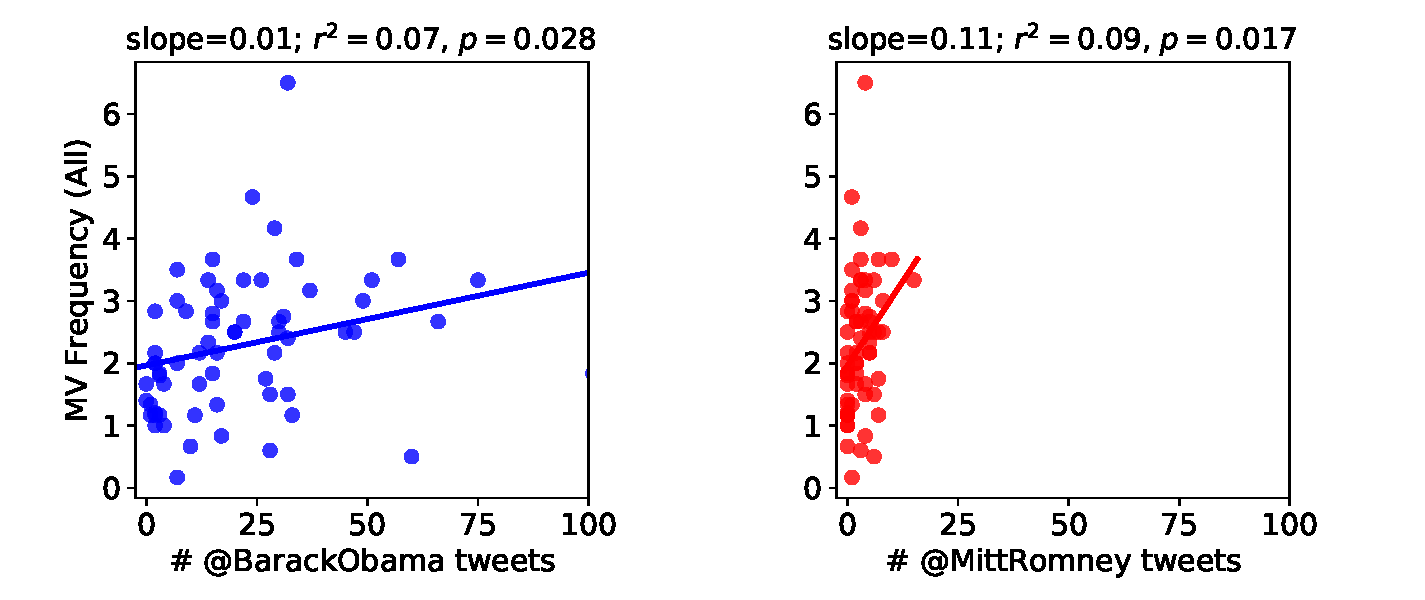
\includegraphics[width=\textwidth]{Figures/2012-all.pdf}
      \caption{2012}
      \label{fig:2012-all-reg}
    \end{subfigure} \\[2em]
    \begin{subfigure}{0.9\linewidth}
      \centering
      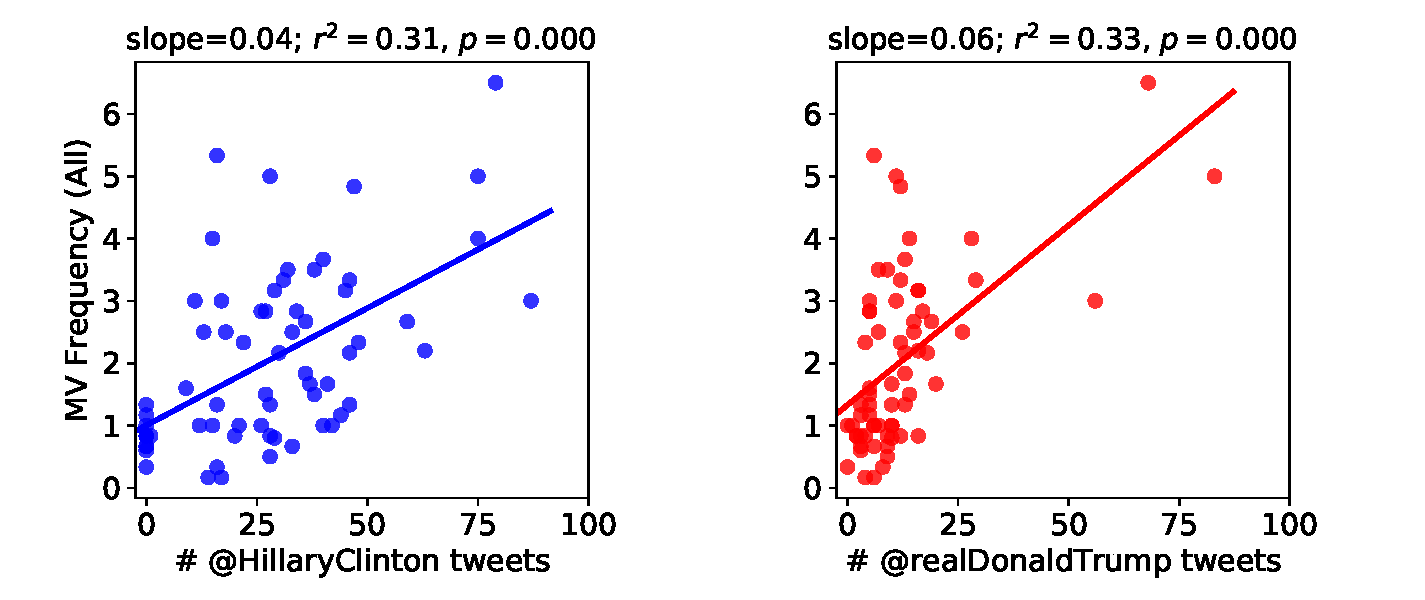
\includegraphics[width=\textwidth]{Figures/2016-all.pdf}
      \caption{2016}
      \label{fig:2012-all-reg}
    \end{subfigure}
  \caption{Metaphorical violence tracked candidate tweets significantly in 2012 and
    2016. Frequency is over all networks and subject/object relationships.
    Correlation coefficient is greater in 2016 than 2012, supporting other 
    claims of 2016 being a ``Twitter election.''
  }
  \label{fig:regressions-all}
\end{figure}


\begin{figure}[h]
  \centering
    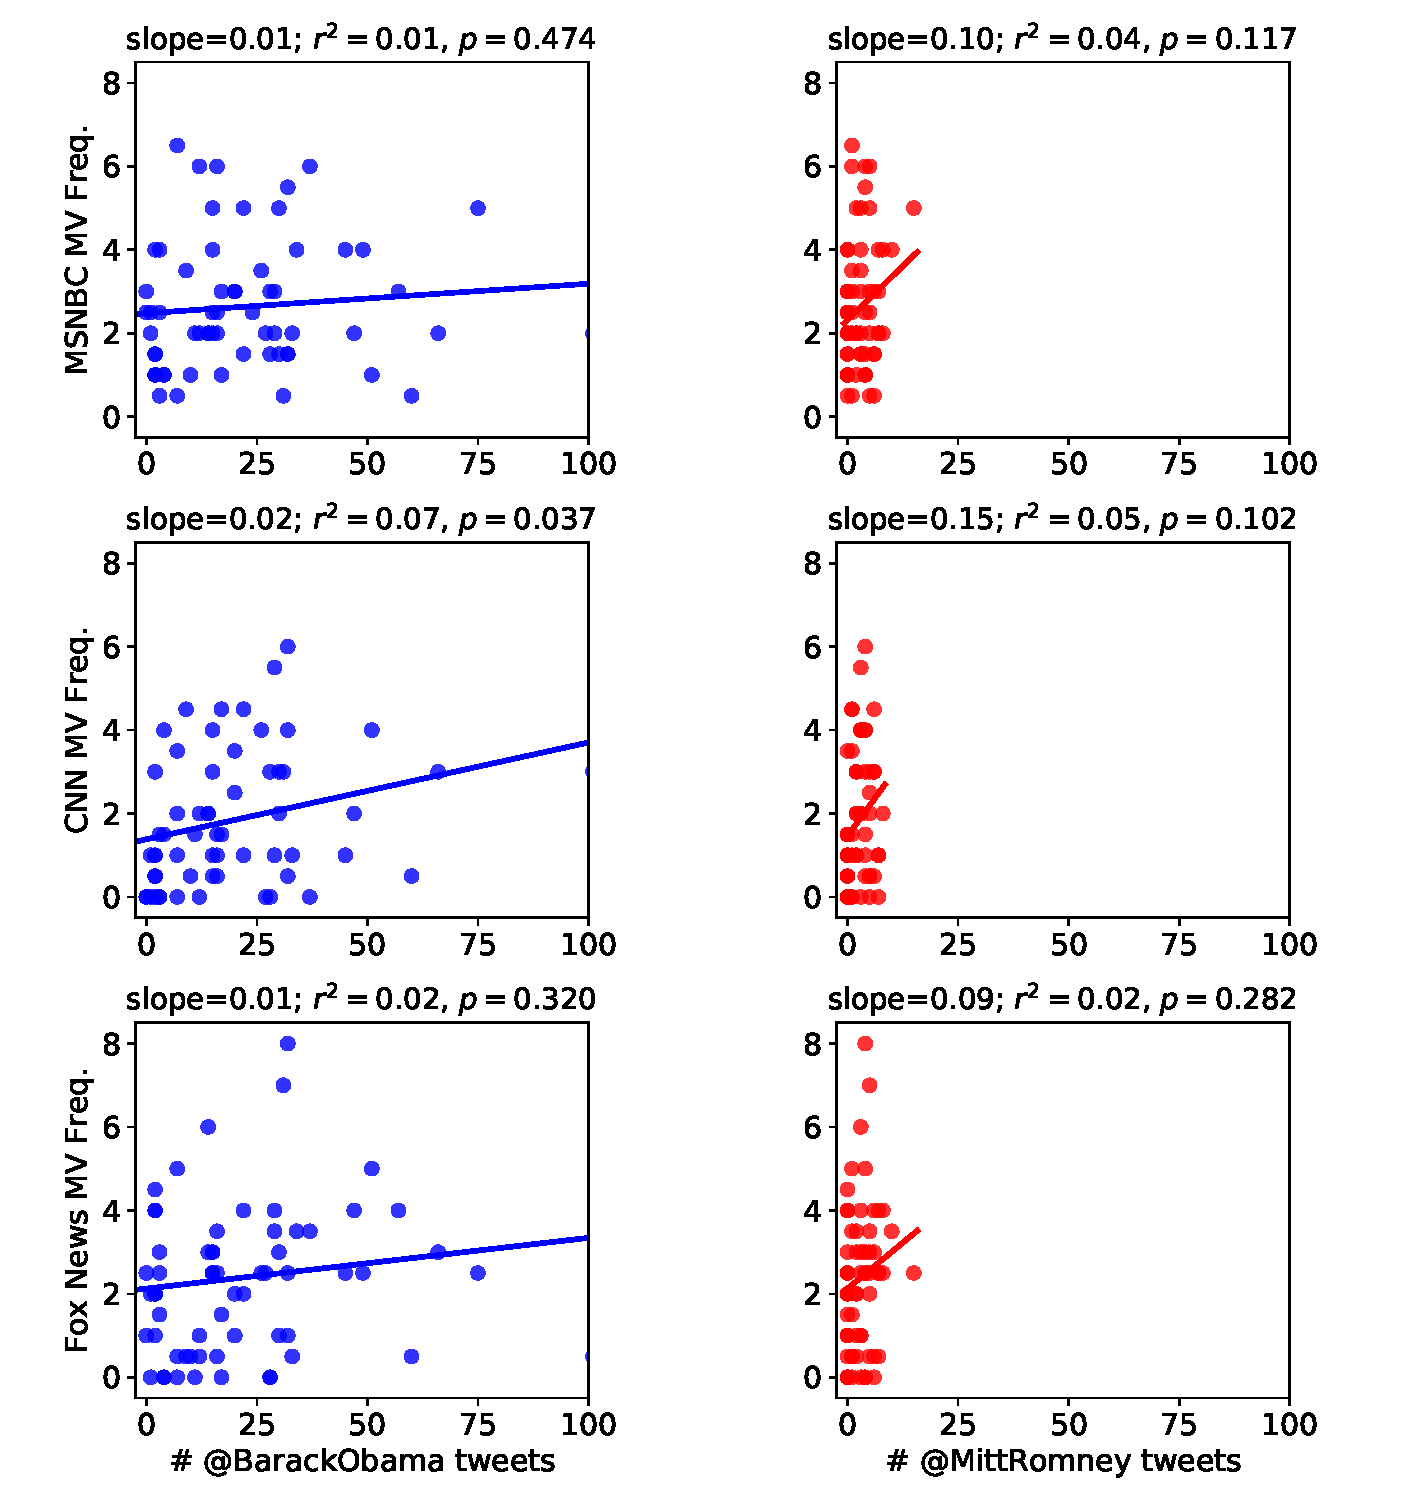
\includegraphics[width=0.95\textwidth]{Figures/2012-network.pdf}
  \caption{Regressions of metaphorical violence on each network in response
   to tweets from @BarackObama and @MittRomney.}
  \label{fig:2012-network}
\end{figure}


\begin{figure}[h]
  \centering
    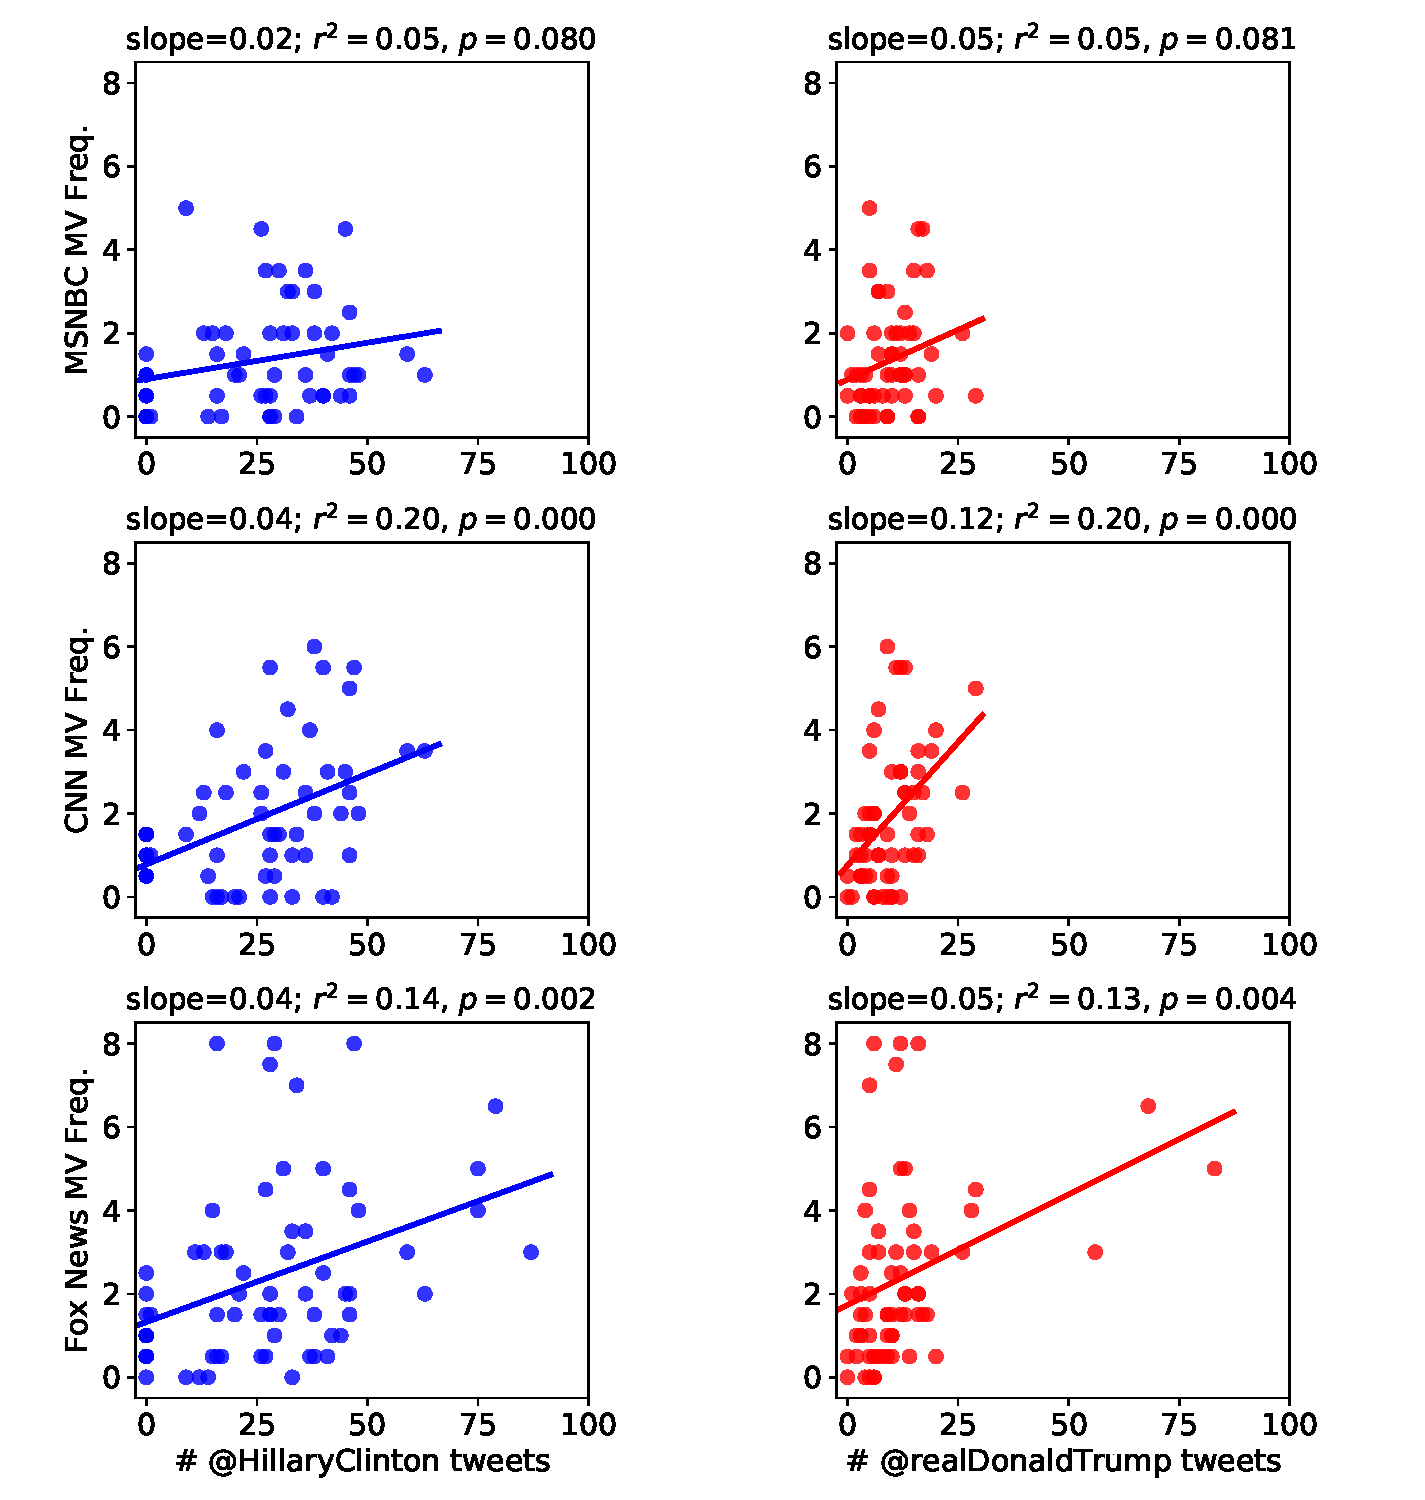
\includegraphics[width=0.95\textwidth]{Figures/2016-network.pdf}
  \caption{Regressions of metaphorical violence on each network in response
   to tweets from @HillaryClinton and @realDonaldTrump.}
  \label{fig:2016-network}
\end{figure}


\begin{figure}[h]
  \centering
    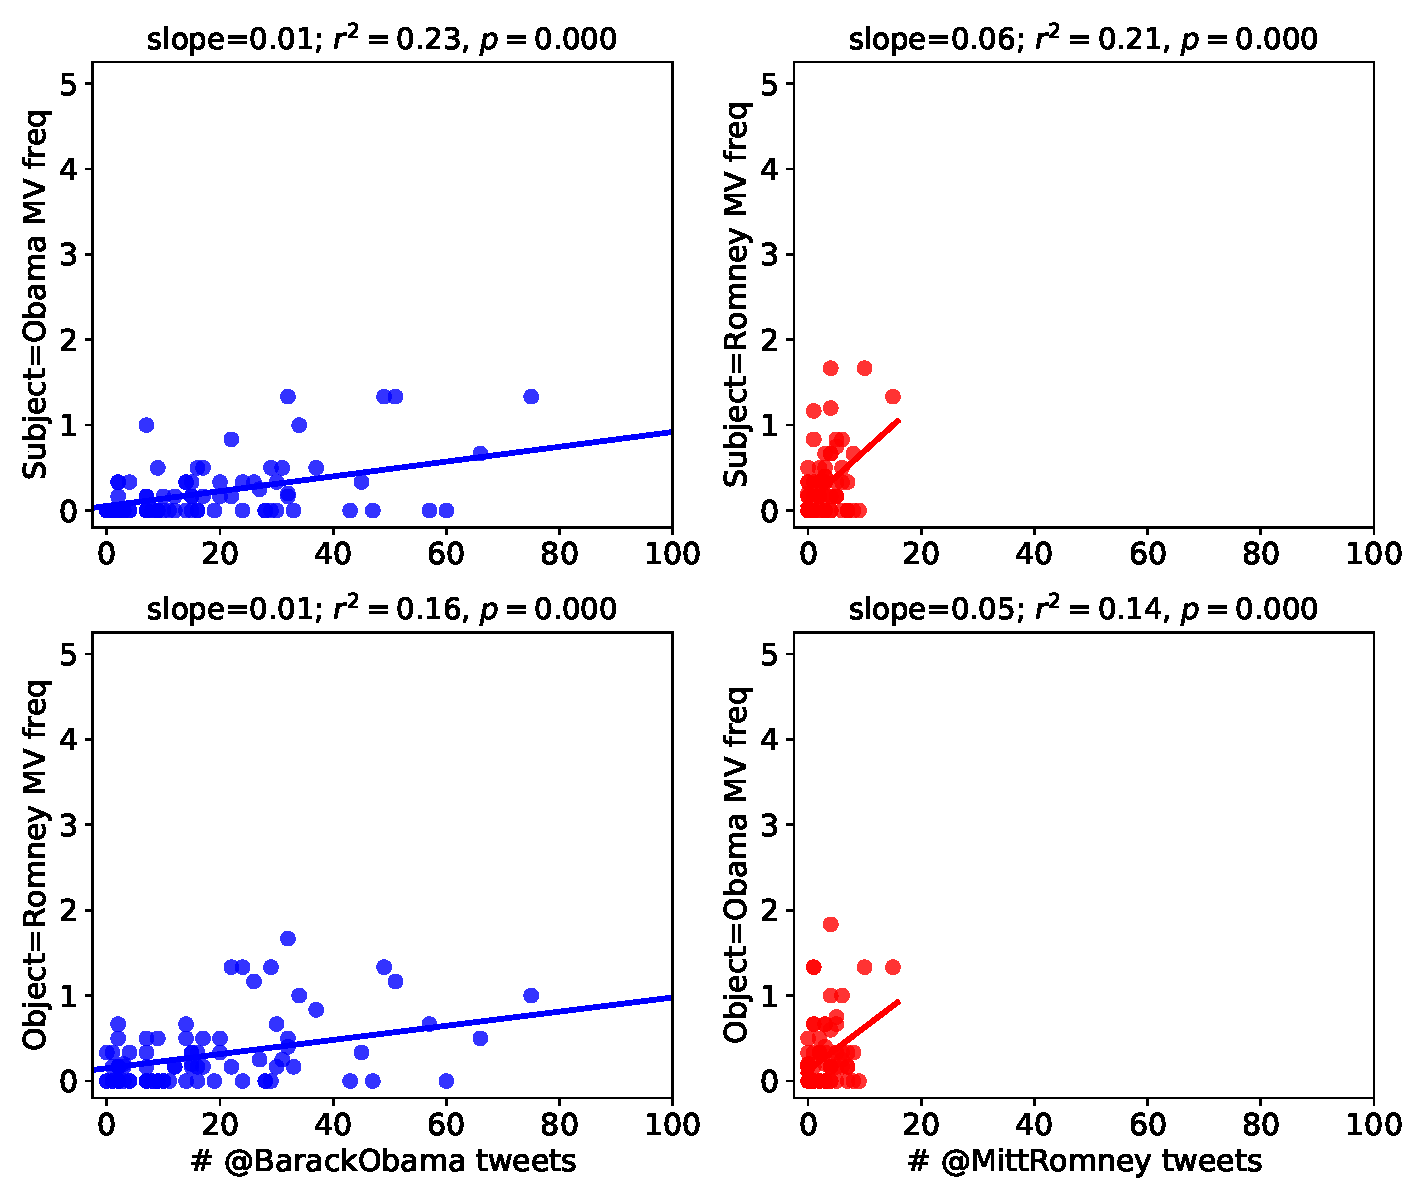
\includegraphics[width=0.9\textwidth]{Figures/2012-subjobj.pdf}
  \caption{Regressions of metaphorical violence faceted by subject and object
    in response to to tweets from @BarackObama and @MittRomney.}
  \label{fig:2012-subjobj}
\end{figure}


\begin{figure}[h]
  \centering
    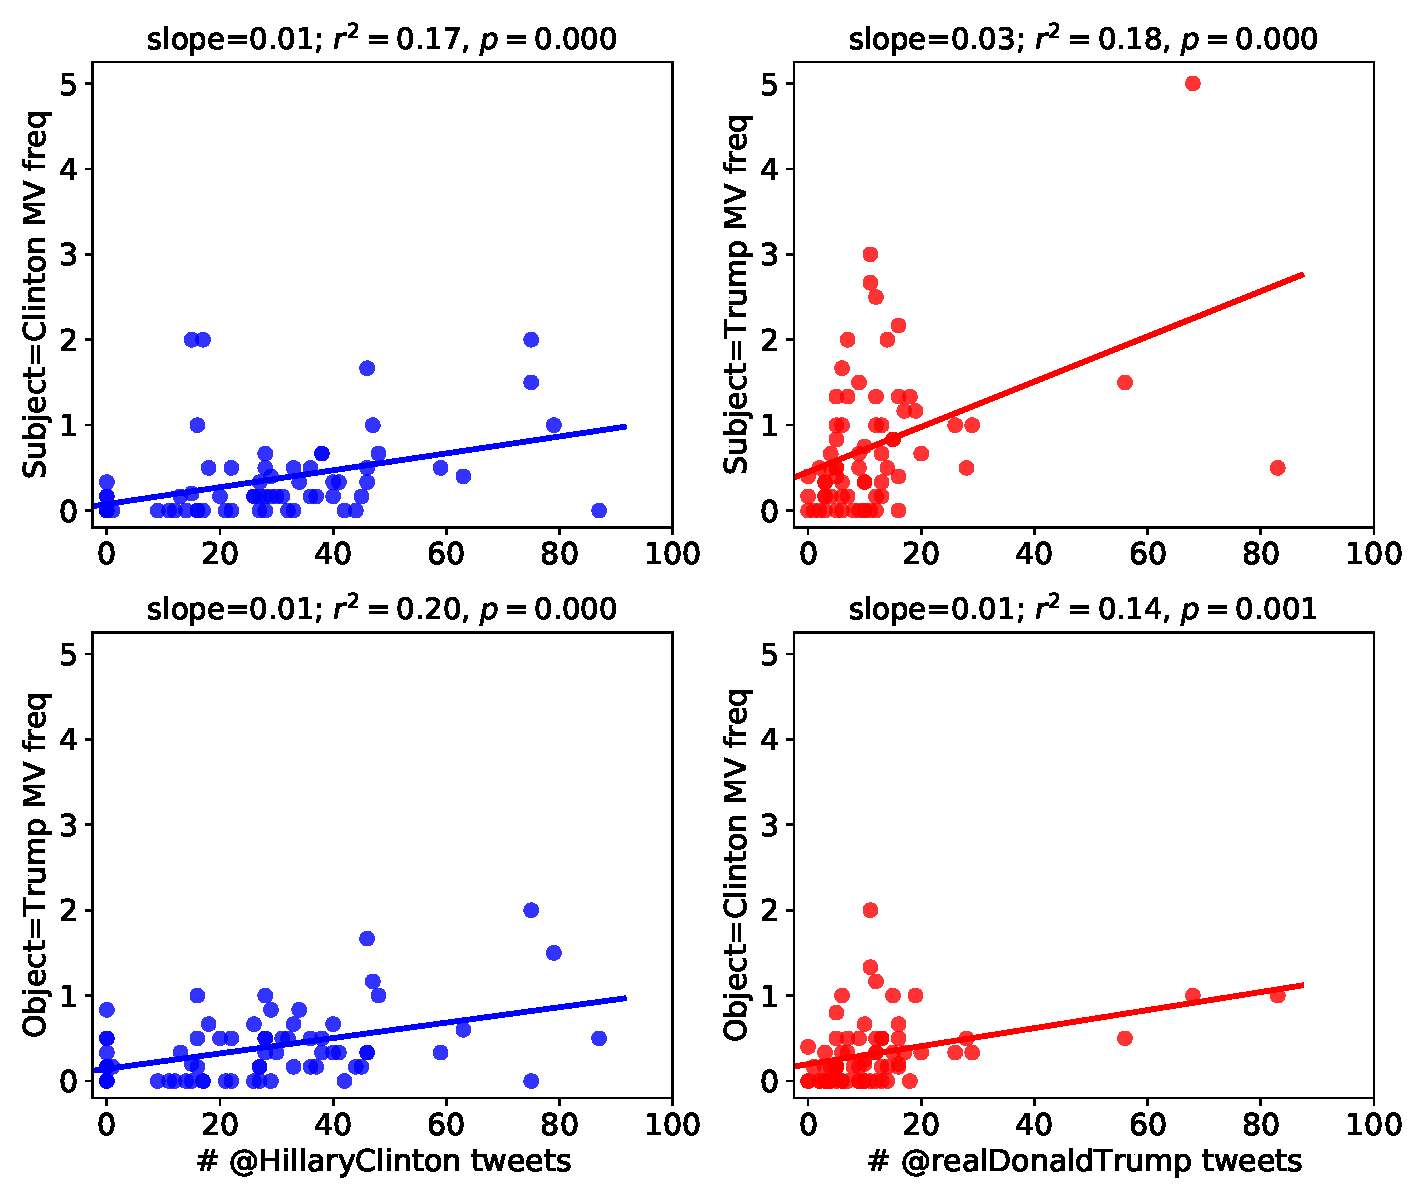
\includegraphics[width=0.9\textwidth]{Figures/2016-subjobj.pdf}
  \caption{Regressions of metaphorical violence faceted by subject and object
    in response to to tweets from @HillaryClinton and @realDonaldTrump.}
  \label{fig:2016-subjobj}
\end{figure}



%%
% Table with regression coefficients, r^2, and p-values for MV vs. tweets
% from all candidates in both years.
%
\begin{table}[h]
  \centering
  \begin{tabular}{lllll}
  \toprule
                    & \multicolumn{4}{c}{(Reg. coefficient, $r^2$) for tweets from} \\
  Met. Vi. Category & @BarackObama & @MittRomney & @HillaryClinton & @realDonaldTrump \\
  \midrule
  All               & (0.01, 0.07)** & (0.11, 0.09)** & (0.04, 0.31)*** & (0.06, 0.33)*** \\
  \hline
  MSNBC             & (0.01, 0.01)   & (0.10, 0.04) &  (0.02, 0.05)* &  (0.05, 0.05)* \\
  CNN               & (0.02, 0.07)** & (0.15, 0.05) &  (0.04, 0.20)*** &  (0.12, 0.20)*** \\
  Fox News          & (0.01, 0.02)   & (0.09, 0.02) &  (0.04, 0.14)** &  (0.05, 0.13)*** \\
  \hline
  Self as subject   & (0.01, 0.23)***   & (0.06, 0.21)*** &  (0.01, 0.17)*** &  (0.03, 0.18)*** \\
  Other as object   & (0.01, 0.16)***   & (0.05, 0.14)*** &  (0.01, 0.20)*** &  (0.01, 0.14)*** \\
  \bottomrule
  \multicolumn{5}{r}{*p<0.1; **p<0.05; ***p<0.01}
\end{tabular}

  \caption{Regression coefficients, $r^2$, and significance indicators for
    linear models of metaphorical violence usage as a function of the number of
    tweets from individual candidates. The regression
    coefficient represents the additional metaphorical violence uses that 
    occur with each message the candidate tweets. $r^2$ represents the fraction
    of variance that is represented through a linear relationship with candidate
    tweets. The 2016 candidates's Twitter use had a greater impact on metaphorical
    violence usage than the 2012 candidates's. In both years, Twitter use 
    had a strong effect on metaphorical violence use where the tweeting candidate was
    cast as the subject of metaphorical violence, or where the other candidate
    was the object of metaphorical violence.}
  \label{tab:twitter-regr-results}
\end{table}
